\documentclass{report} 

\usepackage{amsmath} % \usepackage is a command that allows you to add functionality to your LaTeX code
\usepackage{graphfig, subfig}
\usepackage{graphicx}
\usepackage{hyperref}

\usepackage{geometry}
\geometry{
a4paper,
 total={170mm,257mm},
 left=20mm,
 top=20mm,
}


\usepackage{caption}
\captionsetup{labelformat=empty,textfont=sl}

\usepackage[Glenn]{fncychap}
\title{Storytelling} % Sets article title
\author{Emmanuele Virginio Coppola, Muriel Rossi, Alessandro Marigliano} % Sets authors name

\begin{document} % All begin commands must be paired with an end command somewhere 
    \maketitle % creates title using information in preamble (title, author, date)  $\downarrow$   \date{\today} % Sets date for date compiled

    \tableofcontents
    \chapter{Introduzione} % creates a chapter
    
    La pubblicità invasiva si rivela essere sempre maggiormente un problema asfissiante all'interno del mondo dei socialnetwork. Nonostante siano state sviluppate diverse tecniche
    allo scopo di domare questa piaga, alcune inserzioni riescono tuttavia a sfuggirne, intasando interfacce dedicate all'informazione ed 
    all'intrattenimento, che subiscono così una svalutazione, venendo "soffocate".
    

    \textbf{Legge di Reed: il valore di una rete sociale è direttamente proporzionale ad una funzione esponenziale in N:}
    \begin{equation} % Creates an equation environment and is compiled as math
        V=a*N+b*N^2 + c*2^n
    \end{equation}
    

    La legge sopra citata, descrive come il valore di una rete, formata da interazioni ed intrecci, cresca esponenzialmente con la dimensione di quest'ultima. (1.1).
    In particolare, nel caso di Internet, si osserva come il suo valore tenda a crescere in modo esponenziale se associato a gruppi con interessi
     comuni, che condividono idee, interessi ed obiettivi.
    Da questo se ne deduce come invece, avvisi pubblicitari, spam ed altra "informazione spazzatura", possano far decadere il valore di una rete.
    
    Questo progetto si prefigge lo scopo di manutenere una piattaforma libera dal bombardamento pubblicitario e dare modo all'utenza di potersi esprimere liberamente
    all'interno di questa, distaccandosi dall'ansia e dalla continua distrazione provocata dal chiasso delle inserzioni.
    \chapter{Descrizione dell'agente}
    Allo scopo di realizzare questo progetto, è stato introdotto un agente intelligente, sarà lui ad occuparsi della supervisione della piattaforma, indagando fra i 
    commenti relativi alle varie pubblicazioni.
    \section{Obiettivi}
    L'obiettivo dell'agente sarà quello di effettuare un'analisi giornaliera dei commenti relativi ad ogni pubblicazione effettuata dagli utenti della piattaforma.
    Il testo dei vari commenti verrà preso in analisi e, dopo essere stato adeguatamente "pulito", verrà sottoposto all'agente, che sarà in grado di riconoscere se il 
    testo è conforme alle norme della piattaforma (ovvero se non è sospettato come spam). \newline
    In caso negativo, l'autore del commento verrà segnalato alla piattaforma, che provvederà ad eliminarlo da quest'ultima, assieme a tutto il materiale da lui pubblicato.

    \section{Specifiche PEAS}
    Le specifiche PEAS rappresentano diverse proprietà tramite cui è possibile descrivere l'agente. \newline

    \begin{itemize}
        \item 
        {\bfseries P = Performance.} 
        L'agente verrà valutato in base alla percentuale di commenti spam categorizzati correttamente.
        \item 
        {\bfseries E = Environment.} L'agente nel caso in questione lavorerà su query di commenti relativi ai post pubblicati sul Social Network, 
        navigando fra i commenti degli utenti.\newline
        Nello specifico l'ambiente sarà:
            \begin{itemize}
                \item {\bfseries Completamente Osservabile}, in ogni momento l'agente ha completa conoscenza
                dell'ambiente in cui lavora, ovvero la collezione di commenti;
                \item {\bfseries Deterministico}, l'ambiente verrà modificato in base alla decisione dell'agente, 
                ovvero verranno rimossi gli utenti che l'agente deciderà di segnalare;
                \item {\bfseries Episodico}, l'agente viene attivato ad intervalli temporali di 24h. La scelta che compirà l'agente in un singolo episodio dipenderà dall'episodio stesso;
                \item {\bfseries Statico}, mentre analizza la query di commenti, l'ambiente rimane invariato;
                \item {\bfseries Discreto}, l'ambiente infatti fornisce un insieme di parole finite per ogni commento. L'agente
                dovrà decidere orientandosi fra queste ed avrà azioni limitate (segnalare l'utente o non farlo); 
                \item {\bfseries Singolo}, l'agente che opererà sarà singolo.
            \end{itemize}
          
        \item 
        {\bfseries A = Actuators.} L'agente potrà effettuare il suo giudizio stilando una lista di email relative ai proprietari dei commenti che sono stati sospetatti di spam.
        \item 
        {\bfseries S = Sensors.} Il modo in cui l'agente riceverà gli input percettivi sarà tramite il dataset di commenti.I sensori attraverso cui riceve gli input percettivi.
        
    \end{itemize}
    

    

                        


   
    \chapter{Raccolta, analisi e preprocessing dei dati}
    L'agente, prima di essere inserito all'interno della piattaforma, è stato "allenato" su un dataset, scelto accuratamente per massimizzare la somiglianza ai dati con cui dovrà lavorare 
    durante la sua effettiva applicazione. 
    \section{Scelta del dataset}
    Il dataset preso in esame viene composto da query di commenti relativi a diversi video sulla piattaforma di streaming YouTube. 
    Consiste in un insieme di tuple presentanti le colonne:
    \begin{itemize}

        \item "COMMENT\textunderscore ID"

        \item "AUTHOR", l'autore
        \item "DATE", la data in cui è stato pubblicato
        \item "CONTENT", il suo contenuto
        \item "CLASS", contenente un numero (0 o 1), che individua il commento come ham o spam rispettivamente.
    \end{itemize}

    
    \begin{figure}[h]

        \centering
        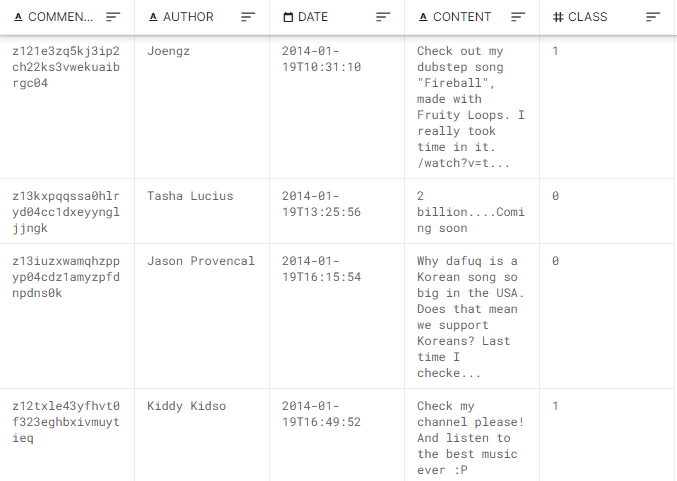
\includegraphics[width = 0.8\textwidth]{immagini/datasetExample.png}
        \caption{Immagine di uno dei dataset iniziali}

    \end{figure}


    E' stato scelto questo dataset in quanto i commenti susseguenti i video si avvicinavano estremamente alle possibili tuple di commenti
    di un reale caso applicativo all'interno della piattaforma.
    Inoltre presentava un'amplia gamma di instanze, così da permettere un buon addestramento dell'agente.
    Le query di commenti sono state trovate a questo indirizzo: \newline 
    \href{https://www.kaggle.com/datasets/lakshmi25npathi/images}{https://www.kaggle.com/datasets/lakshmi25npathi/images}.
    
    \section{Pulizia del dataset}
    Il dataset, nonostante fosse già estremamente adeguato alle esigenze dell'agente, durante la fase di feature extraction, 
    è stato privato della colonne: "COMMENT\textunderscore ID", "AUTHOR", "DATE", in quanto avrebbero potuto falsare i risultati dell'agente, 
    perchè non inerenti all'identificazione di un commento spam.
    L'operazione di pulizia si è poi composta delle seguenti fasi: 

    \begin{itemize}
        \item {\bfseries Conversione da uppercase a lowercase}, tutte le lettere in maiuscolo sono state convertite in minuscolo;
        \item {\bfseries Rimozione degli invii}, tutti i "break" sono stati rimossi;
        \item {\bfseries Rimozione della punteggiatura}, è stata eliminata ogni forma di punteggiatura;
        \item {\bfseries Trascrizione dei link}, i link sono stati eliminati;
        \item {\bfseries Rimozione degli spazi}, gli spazi consecutivi, ovvero in  quantità maggiore di 1, sono stati rimossi;
        \item {\bfseries Eliminazione lettere ripetute}, lettere identiche, ripetute in quantità maggiore di 2, sono state rimosse;
        \item {\bfseries Correzione delle parole}, parole non presenti all'interno del vocabolario inglese di Word Reference (scritte quindi in maniera errata oppure in tempi diversi dall'infinito), sono state sottoposte 
        ad un algoritmo di pattern matching. La funzione nello specifico, cerca inizialmente il match con parole di uso più comune. Il caso in cui
        la parola presenti più matches, viene scelta la prima parola ad essere stata individuata;
        \item {\bfseries Eliminazione delle "stopwords"}, tutte le parole che rientravano nel dizionario delle stopwords (ovvero parole che non aggiungono alcuna informazione) 
        sono state eliminate;
        \item {\bfseries Eliminazione valori nulli}, tutti i testi che, dopo aver superato questa scrematura, risultavano infine vuoti, sono stati eliminati.

 
    \end{itemize}
    \newpage
    
   

    \section{Bilanciamento del dataset}
    
    
    Questo è il grafico della suddivisione fra spam ed ham nei vari dataset.
    \begin{figure}[h]
        \centering
        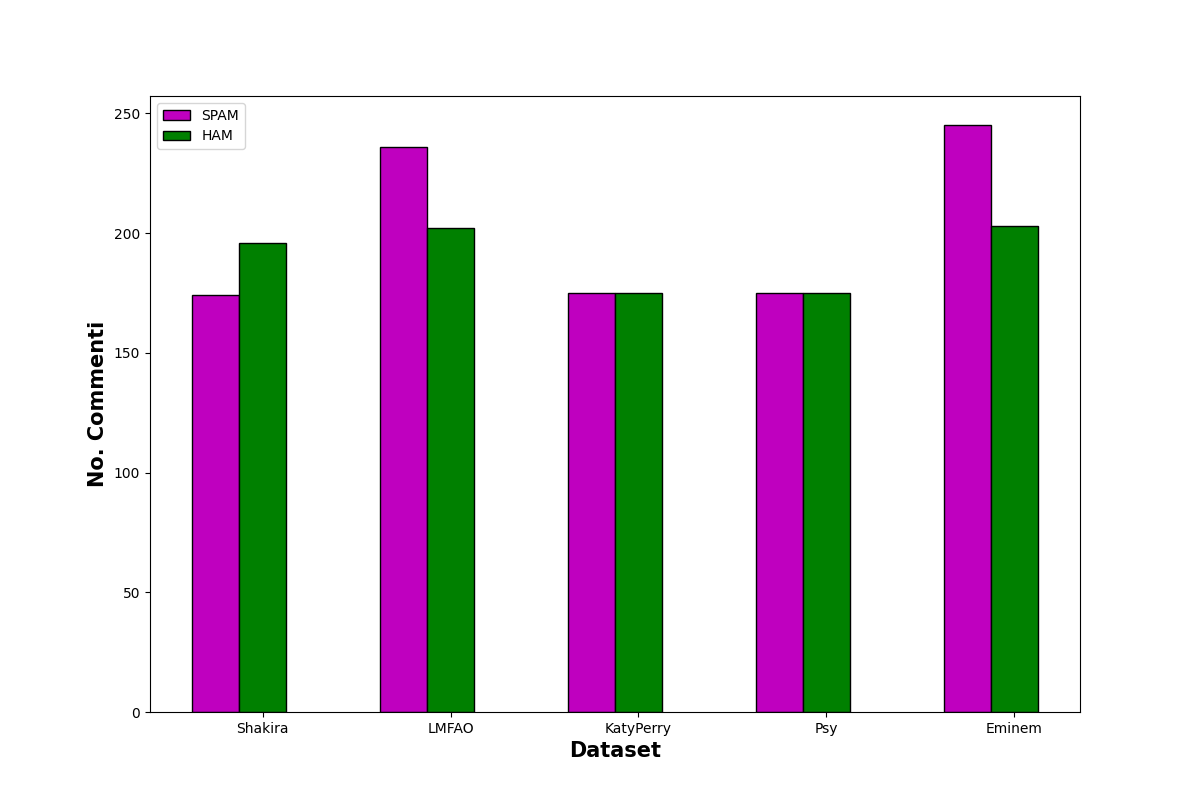
\includegraphics[width = \textwidth]{immagini/DatasetSeparati.png}

    \end{figure}

    Questo è il grafico della suddivisione fra spam ed ham in tutti i dataset.


    \begin{figure}[h!]
        \centering
        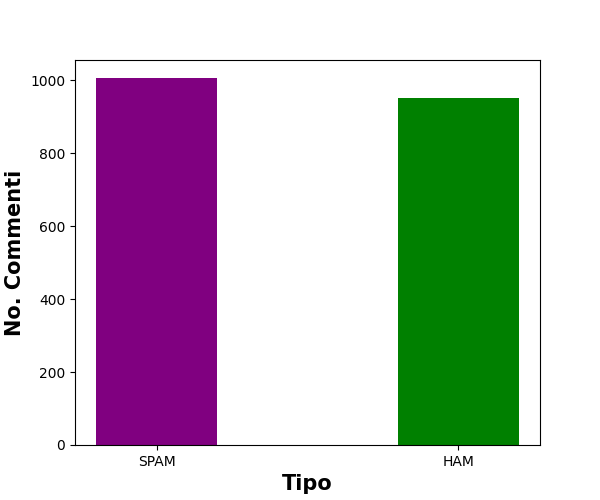
\includegraphics[height = 0.6\textwidth]{immagini/DatasetUnico.png}
    \end{figure}



    \chapter{Creazione agente}
    \section{Addestramento}
    Prima di poter addestrare l'agente, il dataset è stato sottoposto all'operazione di vettorizzazione, che consiste in due fasi:
    \begin{itemize}
        \item separazione del materiale testuale in un vettore contenente le singole parole (tokenizzazione);
        \item traduzione delle parole in numeri, rappresentanti la frequenza della parola all'interno del vettore iniziale.
    \end{itemize}
    A questo scopo è stata utilizzata la libreria "CounterVectorizer".
    \newline
    Una volta terminata questa fase, il dataset è stato suddiviso in 2 insiemi:
    \begin{itemize}
        \item {\bfseries Training Set}: la parte del dataset riservata all'addestramento dell'agente. E' stata costituita dal 
        70\% del dataset totale.
        \item {\bfseries Testing Set}: la parte del dataset riservata al testing dell'agente. Questo set di tuple è stato 
        costituito dal 30\% del dataset totale.
    \end{itemize}
    L'addestramento è stato effettuato su diversi tipi di classificatori, in modo da poter selezionare il migliore in fase di testing.
    I vari classificatori sono stati reperiti dalla libreria: \href{https://scikit-learn.org/stable/modules/naive_bayes.html}{https://scikit-learn.org/stable/modules/naive\textunderscore bayes.html}
    ed è stata utilizzata la versione 1.1.1.
    Nello specifico, ci si è concentrati principalmente su classificatori Naïve Bayes in quanto la loro applicazione risulta consigliata
    su decisioni inerenti a brevi testi, in oltre risultano essere molto rapidi sia in fase di addestramento che in fase di esecuzione.
    Nello specifico sono stati messi a confronto i classificatori:
    \begin{itemize}
        \item {\bfseries GaussianNB}
        \item {\bfseries BernulliNB}
        \item {\bfseries ComplementNB}
        \item {\bfseries MultinomialNB}
    \end{itemize}

    \begin{figure}[h!]
        \centering
        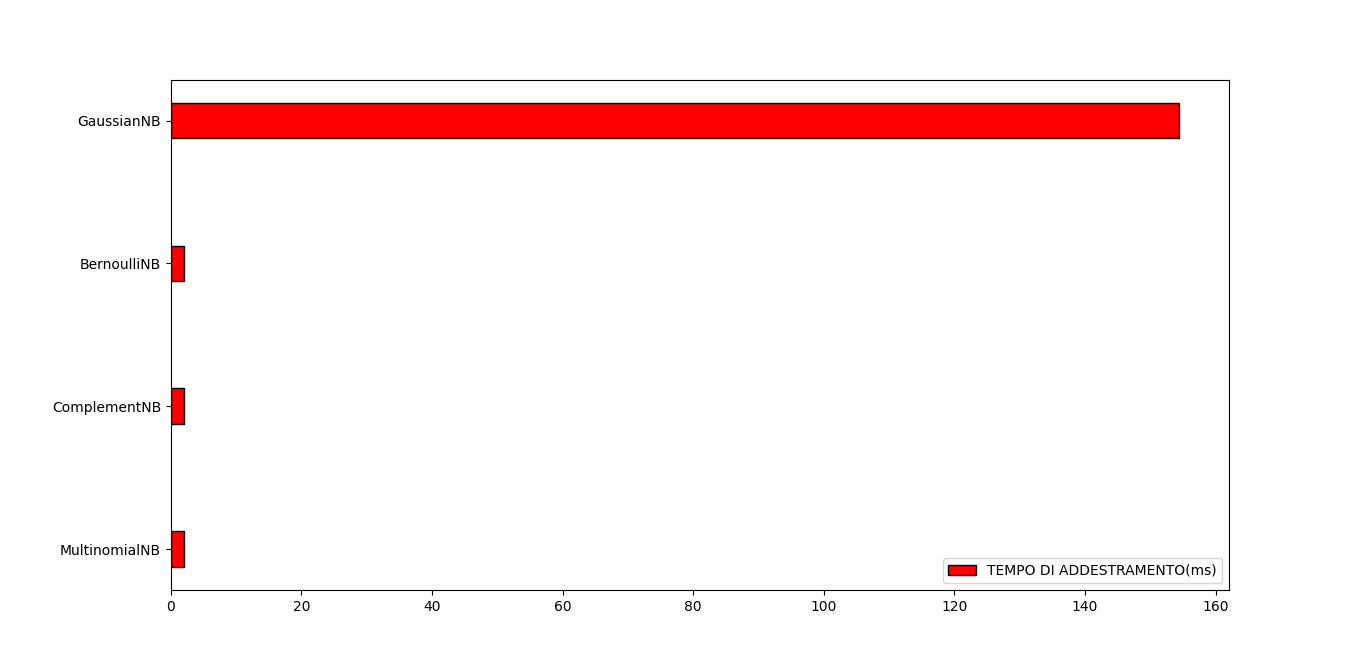
\includegraphics[width =\textwidth]{immagini/graficoAddestramento.png}
        \caption{Grafico che rappresenta i tempi di addestramento di diversi algoritmi Naïve Bayes}

    \end{figure}

    In questa fase, il GaussianNB è risultato essere il più lento in fase di addestramento.


    
    
\newpage
    \section{Testing}
    Durante la fase di testing, i vari classificatori selezionati sono stati eseguiti sullo stesso Testing Set.
    I parametri che hanno influito nella scelta del classificatore da utilizzare sono stati:
    \begin{itemize}
        \item {\bfseries precision}, indica la quantità di previsioni corrette rispetto a tutte le istanze che ha classificato come spam;
        \item {\bfseries recall}, indica quante, fra tutte le istanze spam contenute nel Testing Set, sono state correttamente classificate come spam;
        \item {\bfseries accuracy}, indica il numero totale di previsioni giuste, fra spam ed ham;
        \item {\bfseries MCC}, è un coefficiente che si aggira fra 1 e -1. Questo intero rappresenta la media delle precisioni, dove per 1 
        si intende che il classificatore fa sempre la scelta giusta, mentre per -1 si intende che classifica sempre il contrario della realtà.  
    \end{itemize}

  
        \begin{figure}[h]
            \centering
            \includegraphics[width =\textwidth]{immagini/graficoBuono.png}
            \caption{Grafico che rappresenta vari parametri di diversi algoritmi Naïve Bayes}

        \end{figure}
        
        Oltre ai parametri sopra elencati, è stato considerato anche il tempo di esecuzione.
        In questo caso il GaussianNB è risultato essere il più lento ad essere eseguito.
        \newpage
        
        \begin{figure}[h]
            \centering
            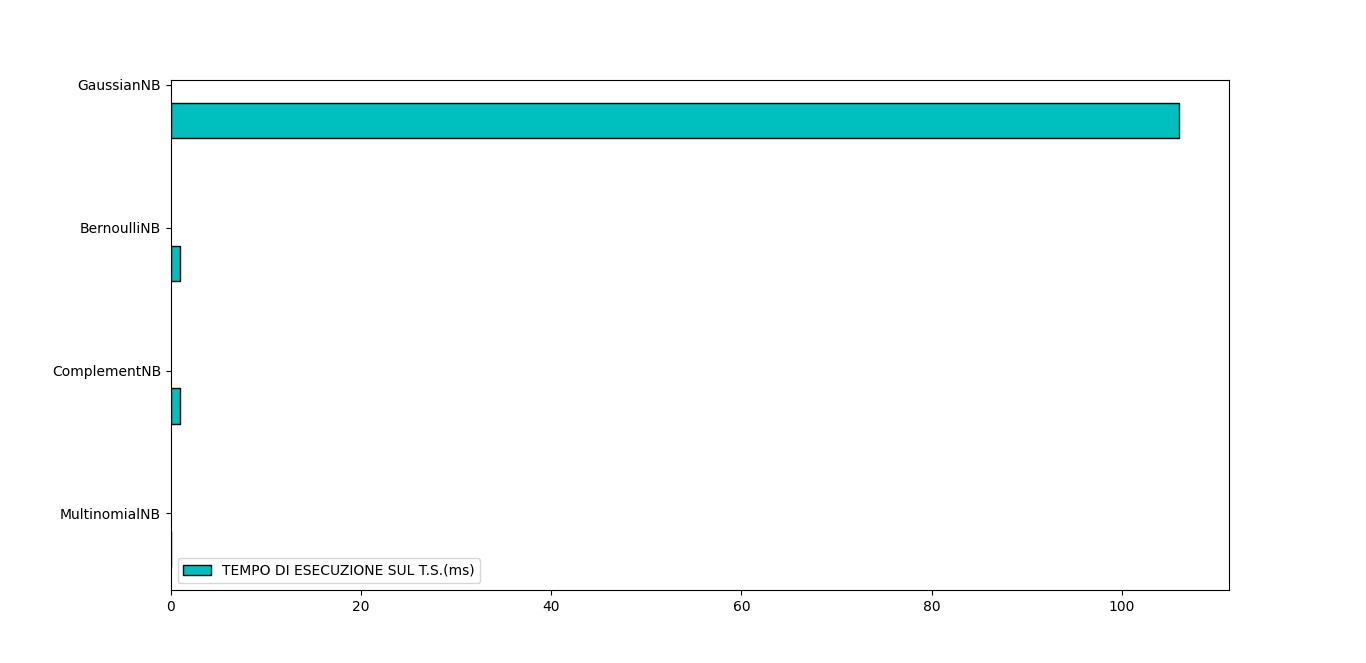
\includegraphics[width =\textwidth]{immagini/graficoEsecuzione.png}
            \caption{Grafico che rappresenta il tempo di esecuzione sul Testing Set di diversi algoritmi Naïve Bayes}
        \end{figure}

    I vari test sono stati ripetuti anche modificando il Random State: il parametro che permette di ottenere un mescolamento e 
    un suddivisione tra training e testing set ripetibile nelle varie chiamate.
    Il valore ottimale del RandomState si è rivelato essere 42.
    

    \begin{figure}[h]
            \centering
            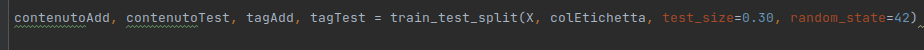
\includegraphics[width =\textwidth]{immagini/randomState.png}
            \caption{Immagine di come è stato modificato il Random State in modo da essere ottimizzato}

    \end{figure}

                
    In base ai vari parametri mostrati in precedenza, è stato scelto di adottare il ComplementNB come modello per l'agente.
    risultato il ComplementNB che ha battuto per poche classificazioni corrette e per pochi millisecondi
        in meno di esecuzione il MultinomialNB, battendo anche il BernoulliNB che per documentazione 
        di scikit-learn dovrebbe essere migliore per documenti corti.

    
        \section{Scelta del modello}
    
        Dopo aver definito gli obiettivi dell'agente, le sue specifiche, l'ambiente in cui avrebbe lavorato, ed il suo dataset, si è deciso come andava effettivamente costruito l'agente.
        L'agente dovrà stimare se un commento è un avviso pubblicitario o meno con il solo aiuto delle parole presenti nel commento. Inizialmente è stato sottoposto all'agente 
        un dataset di commenti, ognuno dei quali è contrassegnato da un intero che rappresenta la classe a cui appartiene l'elemento "1", se lo specifico commento è, o contrassegnato da classe "0" se il commento è ham.
        E' quindi stata creata una tabella dove venivano individuate, per ciascun commento,
        la frequenza con la quale alcune parole ricorrevano. In questo caso ci è venuto in aiuto l'algoritmo {\bfseries Naive Bayes}:
        \newline
        \begin{equation}\label{bho}
            { p(B|A)  p(A)\over p(B)}
        \end{equation}
        \newline
        che, nel nostro caso, si traduce in:
        \newline
        \begin{equation}\label{bho2}
            p(spam|commento) = { p(commento|spam)  p(spam)\over p(commento)}
        \end{equation}
        \newline
        ovvero, la probabilità che un commento sia spam, è uguale alla probabilità che le parole del commento compaiano in un commento spam, dato che è spam, per la probabilità 
        che il commento sia spam, diviso la probabilità che queste parole compaiano nel commento.
    
    

    \chapter{Esecuzione agente}
    
    L'agente, per poter essere eseguito, deve essere integrato all'interno della piattaforma Storytelling.
    I due sistemi dovranno poter comunicare nonostante siano stati formulati in linguaggi diversi.
    \newline
    A questo scopo sono state utilizzate delle tecniche che, oltre a essere funzionali per la piattaforma in questione,
    hanno reso più agevole l'integrazione dell'agente anche in altre piattaforme, scritte in qualsivoglia linguaggio.

    \section{Prelevamento istanze}
    Il sistema di comunicazione fra l'agente e la piattaforma, essendo scritte rispettivamente in Python 3.10 ed in Java 15.0.2, è stato 
    implementato tramite una socket, sulla quale l'agente ogni 24h:
    \begin{itemize}
        \item si avvia ad un orario prestabilito;
        \item rimane in attesa, fino alla ricezione della richiesta di Storytelling;
        \item riceve dalla socket la lista di commenti da analizzare, in formato JSON, assieme al loro corrispettivo autore;
        \item li inserisce in un dataframe generato tramite la libreria Pandas ed esegue le operazioni di pulizia, avviandola su processi differenti;
        \item esegue la classificazione;
        \item inoltra sulla socket i nominativi degli autori dei commenti che sono stati classificati come spam;
        \item chiude la socket e si termina la sua esecuzione;
    \end{itemize}

    \begin{figure}[h!]
        \centering
        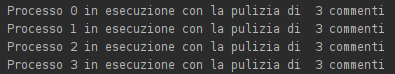
\includegraphics[width =0.5\textwidth]{immagini/puliziaCommenti.png}
        \caption{Avvio dei diversi processi di pulizia in parallelo}

    \end{figure}

    \begin{figure}[h!]
        \centering
        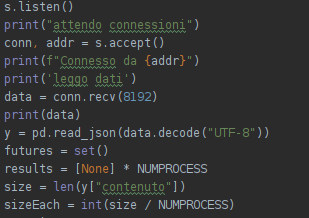
\includegraphics[width =0.4\textwidth]{immagini/socket.png}
        \caption{Immagine di come è stata implementata la comunicazione}

    \end{figure}
    \newpage
    \section{Risultati finali}
    L'agente in campo risulta che performa con una buona precisione ma comunque 

    \begin{figure}[h!]
        \centering
        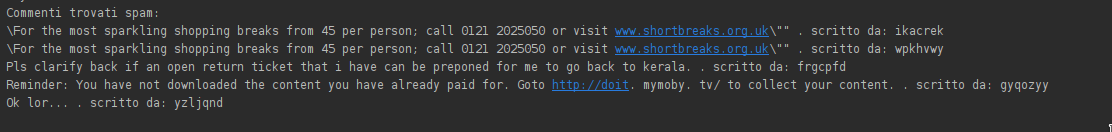
\includegraphics[width =\textwidth]{immagini/commentiSpam.png}
        \caption{Immagine di come è stato modificato il Random State in modo da essere ottimizzato}

\end{figure}



\end{document}
